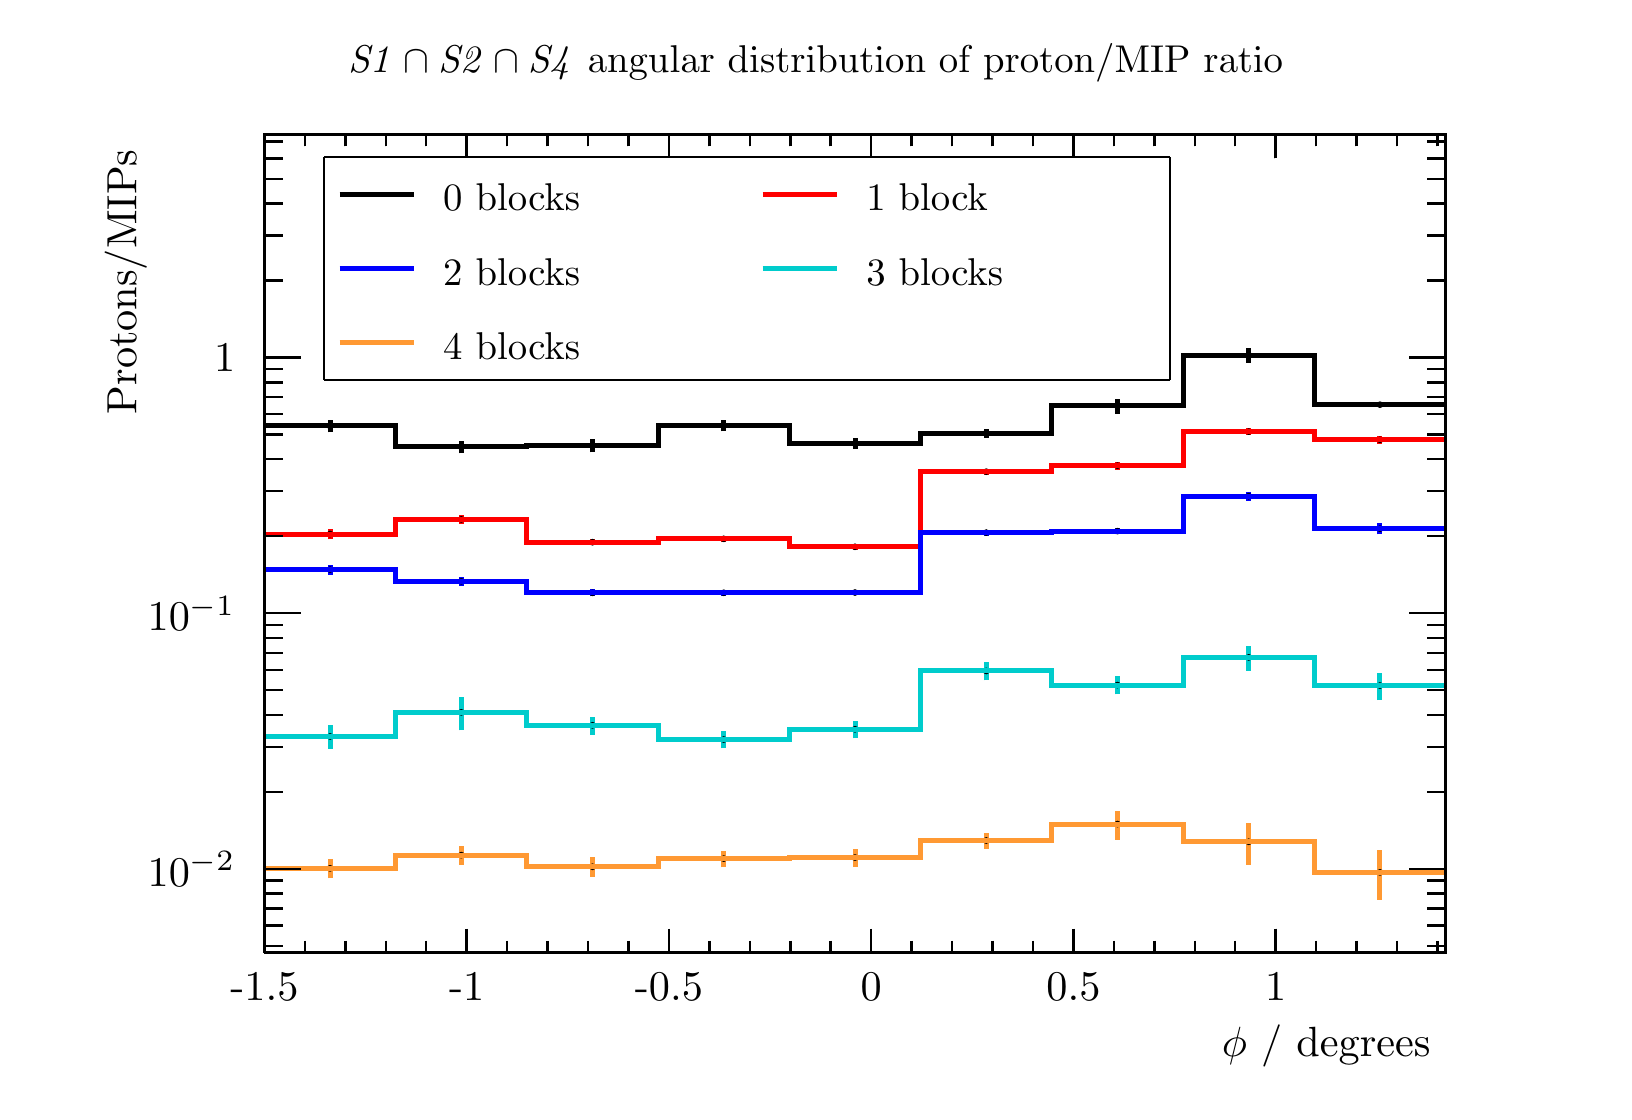
\begin{tikzpicture}
\pgfdeclareplotmark{cross} {
\pgfpathmoveto{\pgfpoint{-0.3\pgfplotmarksize}{\pgfplotmarksize}}
\pgfpathlineto{\pgfpoint{+0.3\pgfplotmarksize}{\pgfplotmarksize}}
\pgfpathlineto{\pgfpoint{+0.3\pgfplotmarksize}{0.3\pgfplotmarksize}}
\pgfpathlineto{\pgfpoint{+1\pgfplotmarksize}{0.3\pgfplotmarksize}}
\pgfpathlineto{\pgfpoint{+1\pgfplotmarksize}{-0.3\pgfplotmarksize}}
\pgfpathlineto{\pgfpoint{+0.3\pgfplotmarksize}{-0.3\pgfplotmarksize}}
\pgfpathlineto{\pgfpoint{+0.3\pgfplotmarksize}{-1.\pgfplotmarksize}}
\pgfpathlineto{\pgfpoint{-0.3\pgfplotmarksize}{-1.\pgfplotmarksize}}
\pgfpathlineto{\pgfpoint{-0.3\pgfplotmarksize}{-0.3\pgfplotmarksize}}
\pgfpathlineto{\pgfpoint{-1.\pgfplotmarksize}{-0.3\pgfplotmarksize}}
\pgfpathlineto{\pgfpoint{-1.\pgfplotmarksize}{0.3\pgfplotmarksize}}
\pgfpathlineto{\pgfpoint{-0.3\pgfplotmarksize}{0.3\pgfplotmarksize}}
\pgfpathclose
\pgfusepathqstroke
}
\pgfdeclareplotmark{cross*} {
\pgfpathmoveto{\pgfpoint{-0.3\pgfplotmarksize}{\pgfplotmarksize}}
\pgfpathlineto{\pgfpoint{+0.3\pgfplotmarksize}{\pgfplotmarksize}}
\pgfpathlineto{\pgfpoint{+0.3\pgfplotmarksize}{0.3\pgfplotmarksize}}
\pgfpathlineto{\pgfpoint{+1\pgfplotmarksize}{0.3\pgfplotmarksize}}
\pgfpathlineto{\pgfpoint{+1\pgfplotmarksize}{-0.3\pgfplotmarksize}}
\pgfpathlineto{\pgfpoint{+0.3\pgfplotmarksize}{-0.3\pgfplotmarksize}}
\pgfpathlineto{\pgfpoint{+0.3\pgfplotmarksize}{-1.\pgfplotmarksize}}
\pgfpathlineto{\pgfpoint{-0.3\pgfplotmarksize}{-1.\pgfplotmarksize}}
\pgfpathlineto{\pgfpoint{-0.3\pgfplotmarksize}{-0.3\pgfplotmarksize}}
\pgfpathlineto{\pgfpoint{-1.\pgfplotmarksize}{-0.3\pgfplotmarksize}}
\pgfpathlineto{\pgfpoint{-1.\pgfplotmarksize}{0.3\pgfplotmarksize}}
\pgfpathlineto{\pgfpoint{-0.3\pgfplotmarksize}{0.3\pgfplotmarksize}}
\pgfpathclose
\pgfusepathqfillstroke
}
\pgfdeclareplotmark{newstar} {
\pgfpathmoveto{\pgfqpoint{0pt}{\pgfplotmarksize}}
\pgfpathlineto{\pgfqpointpolar{44}{0.5\pgfplotmarksize}}
\pgfpathlineto{\pgfqpointpolar{18}{\pgfplotmarksize}}
\pgfpathlineto{\pgfqpointpolar{-20}{0.5\pgfplotmarksize}}
\pgfpathlineto{\pgfqpointpolar{-54}{\pgfplotmarksize}}
\pgfpathlineto{\pgfqpointpolar{-90}{0.5\pgfplotmarksize}}
\pgfpathlineto{\pgfqpointpolar{234}{\pgfplotmarksize}}
\pgfpathlineto{\pgfqpointpolar{198}{0.5\pgfplotmarksize}}
\pgfpathlineto{\pgfqpointpolar{162}{\pgfplotmarksize}}
\pgfpathlineto{\pgfqpointpolar{134}{0.5\pgfplotmarksize}}
\pgfpathclose
\pgfusepathqstroke
}
\pgfdeclareplotmark{newstar*} {
\pgfpathmoveto{\pgfqpoint{0pt}{\pgfplotmarksize}}
\pgfpathlineto{\pgfqpointpolar{44}{0.5\pgfplotmarksize}}
\pgfpathlineto{\pgfqpointpolar{18}{\pgfplotmarksize}}
\pgfpathlineto{\pgfqpointpolar{-20}{0.5\pgfplotmarksize}}
\pgfpathlineto{\pgfqpointpolar{-54}{\pgfplotmarksize}}
\pgfpathlineto{\pgfqpointpolar{-90}{0.5\pgfplotmarksize}}
\pgfpathlineto{\pgfqpointpolar{234}{\pgfplotmarksize}}
\pgfpathlineto{\pgfqpointpolar{198}{0.5\pgfplotmarksize}}
\pgfpathlineto{\pgfqpointpolar{162}{\pgfplotmarksize}}
\pgfpathlineto{\pgfqpointpolar{134}{0.5\pgfplotmarksize}}
\pgfpathclose
\pgfusepathqfillstroke
}
\definecolor{c}{rgb}{1,1,1};
\draw [color=c, fill=c] (0,0) rectangle (20,13.4957);
\draw [color=c, fill=c] (3,1.75444) rectangle (18,12.1461);
\definecolor{c}{rgb}{0,0,0};
\draw [c,line width=0.9] (3,1.75444) -- (3,12.1461) -- (18,12.1461) -- (18,1.75444) -- (3,1.75444);
\definecolor{c}{rgb}{1,1,1};
\draw [color=c, fill=c] (3,1.75444) rectangle (18,12.1461);
\definecolor{c}{rgb}{0,0,0};
\draw [c,line width=0.9] (3,1.75444) -- (3,12.1461) -- (18,12.1461) -- (18,1.75444) -- (3,1.75444);
\draw [c,line width=0.9] (3,1.75444) -- (4.66667,1.75444) -- (4.66667,1.75444) -- (6.33333,1.75444) -- (6.33333,1.75444) -- (8,1.75444) -- (8,1.75444) -- (9.66667,1.75444) -- (9.66667,1.75444) -- (11.3333,1.75444) -- (11.3333,1.75444) -- (13,1.75444)
 -- (13,1.75444) -- (14.6667,1.75444) -- (14.6667,1.75444) -- (16.3333,1.75444) -- (16.3333,1.75444) -- (18,1.75444);
\draw [c,line width=0.9] (3,1.75444) -- (18,1.75444);
\draw [c,line width=0.9] (3,2.05809) -- (3,1.75444);
\draw [c,line width=0.9] (3.5137,1.90627) -- (3.5137,1.75444);
\draw [c,line width=0.9] (4.0274,1.90627) -- (4.0274,1.75444);
\draw [c,line width=0.9] (4.5411,1.90627) -- (4.5411,1.75444);
\draw [c,line width=0.9] (5.05479,1.90627) -- (5.05479,1.75444);
\draw [c,line width=0.9] (5.56849,2.05809) -- (5.56849,1.75444);
\draw [c,line width=0.9] (6.08219,1.90627) -- (6.08219,1.75444);
\draw [c,line width=0.9] (6.59589,1.90627) -- (6.59589,1.75444);
\draw [c,line width=0.9] (7.10959,1.90627) -- (7.10959,1.75444);
\draw [c,line width=0.9] (7.62329,1.90627) -- (7.62329,1.75444);
\draw [c,line width=0.9] (8.13699,2.05809) -- (8.13699,1.75444);
\draw [c,line width=0.9] (8.65069,1.90627) -- (8.65069,1.75444);
\draw [c,line width=0.9] (9.16438,1.90627) -- (9.16438,1.75444);
\draw [c,line width=0.9] (9.67808,1.90627) -- (9.67808,1.75444);
\draw [c,line width=0.9] (10.1918,1.90627) -- (10.1918,1.75444);
\draw [c,line width=0.9] (10.7055,2.05809) -- (10.7055,1.75444);
\draw [c,line width=0.9] (11.2192,1.90627) -- (11.2192,1.75444);
\draw [c,line width=0.9] (11.7329,1.90627) -- (11.7329,1.75444);
\draw [c,line width=0.9] (12.2466,1.90627) -- (12.2466,1.75444);
\draw [c,line width=0.9] (12.7603,1.90627) -- (12.7603,1.75444);
\draw [c,line width=0.9] (13.274,2.05809) -- (13.274,1.75444);
\draw [c,line width=0.9] (13.7877,1.90627) -- (13.7877,1.75444);
\draw [c,line width=0.9] (14.3014,1.90627) -- (14.3014,1.75444);
\draw [c,line width=0.9] (14.8151,1.90627) -- (14.8151,1.75444);
\draw [c,line width=0.9] (15.3288,1.90627) -- (15.3288,1.75444);
\draw [c,line width=0.9] (15.8425,2.05809) -- (15.8425,1.75444);
\draw [c,line width=0.9] (15.8425,2.05809) -- (15.8425,1.75444);
\draw [c,line width=0.9] (16.3562,1.90627) -- (16.3562,1.75444);
\draw [c,line width=0.9] (16.8699,1.90627) -- (16.8699,1.75444);
\draw [c,line width=0.9] (17.3836,1.90627) -- (17.3836,1.75444);
\draw [c,line width=0.9] (17.8973,1.90627) -- (17.8973,1.75444);
\draw [anchor=base] (3,1.14713) node[scale=1.52731, color=c, rotate=0]{-1.5};
\draw [anchor=base] (5.56849,1.14713) node[scale=1.52731, color=c, rotate=0]{-1};
\draw [anchor=base] (8.13699,1.14713) node[scale=1.52731, color=c, rotate=0]{-0.5};
\draw [anchor=base] (10.7055,1.14713) node[scale=1.52731, color=c, rotate=0]{0};
\draw [anchor=base] (13.274,1.14713) node[scale=1.52731, color=c, rotate=0]{0.5};
\draw [anchor=base] (15.8425,1.14713) node[scale=1.52731, color=c, rotate=0]{1};
\draw [anchor= east] (18,0.566819) node[scale=1.52731, color=c, rotate=0]{$\phi$ / degrees};
\draw [c,line width=0.9] (3,12.1461) -- (18,12.1461);
\draw [c,line width=0.9] (3,11.8425) -- (3,12.1461);
\draw [c,line width=0.9] (3.5137,11.9943) -- (3.5137,12.1461);
\draw [c,line width=0.9] (4.0274,11.9943) -- (4.0274,12.1461);
\draw [c,line width=0.9] (4.5411,11.9943) -- (4.5411,12.1461);
\draw [c,line width=0.9] (5.05479,11.9943) -- (5.05479,12.1461);
\draw [c,line width=0.9] (5.56849,11.8425) -- (5.56849,12.1461);
\draw [c,line width=0.9] (6.08219,11.9943) -- (6.08219,12.1461);
\draw [c,line width=0.9] (6.59589,11.9943) -- (6.59589,12.1461);
\draw [c,line width=0.9] (7.10959,11.9943) -- (7.10959,12.1461);
\draw [c,line width=0.9] (7.62329,11.9943) -- (7.62329,12.1461);
\draw [c,line width=0.9] (8.13699,11.8425) -- (8.13699,12.1461);
\draw [c,line width=0.9] (8.65069,11.9943) -- (8.65069,12.1461);
\draw [c,line width=0.9] (9.16438,11.9943) -- (9.16438,12.1461);
\draw [c,line width=0.9] (9.67808,11.9943) -- (9.67808,12.1461);
\draw [c,line width=0.9] (10.1918,11.9943) -- (10.1918,12.1461);
\draw [c,line width=0.9] (10.7055,11.8425) -- (10.7055,12.1461);
\draw [c,line width=0.9] (11.2192,11.9943) -- (11.2192,12.1461);
\draw [c,line width=0.9] (11.7329,11.9943) -- (11.7329,12.1461);
\draw [c,line width=0.9] (12.2466,11.9943) -- (12.2466,12.1461);
\draw [c,line width=0.9] (12.7603,11.9943) -- (12.7603,12.1461);
\draw [c,line width=0.9] (13.274,11.8425) -- (13.274,12.1461);
\draw [c,line width=0.9] (13.7877,11.9943) -- (13.7877,12.1461);
\draw [c,line width=0.9] (14.3014,11.9943) -- (14.3014,12.1461);
\draw [c,line width=0.9] (14.8151,11.9943) -- (14.8151,12.1461);
\draw [c,line width=0.9] (15.3288,11.9943) -- (15.3288,12.1461);
\draw [c,line width=0.9] (15.8425,11.8425) -- (15.8425,12.1461);
\draw [c,line width=0.9] (15.8425,11.8425) -- (15.8425,12.1461);
\draw [c,line width=0.9] (16.3562,11.9943) -- (16.3562,12.1461);
\draw [c,line width=0.9] (16.8699,11.9943) -- (16.8699,12.1461);
\draw [c,line width=0.9] (17.3836,11.9943) -- (17.3836,12.1461);
\draw [c,line width=0.9] (17.8973,11.9943) -- (17.8973,12.1461);
\draw [c,line width=0.9] (3,1.75444) -- (3,12.1461);
\draw [c,line width=0.9] (3.231,1.84239) -- (3,1.84239);
\draw [c,line width=0.9] (3.231,2.09949) -- (3,2.09949);
\draw [c,line width=0.9] (3.231,2.31686) -- (3,2.31686);
\draw [c,line width=0.9] (3.231,2.50516) -- (3,2.50516);
\draw [c,line width=0.9] (3.231,2.67125) -- (3,2.67125);
\draw [c,line width=0.9] (3.462,2.81982) -- (3,2.81982);
\draw [anchor= east] (2.82,2.81982) node[scale=1.52731, color=c, rotate=0]{$10^{-2}$};
\draw [c,line width=0.9] (3.231,3.79726) -- (3,3.79726);
\draw [c,line width=0.9] (3.231,4.36902) -- (3,4.36902);
\draw [c,line width=0.9] (3.231,4.77469) -- (3,4.77469);
\draw [c,line width=0.9] (3.231,5.08935) -- (3,5.08935);
\draw [c,line width=0.9] (3.231,5.34645) -- (3,5.34645);
\draw [c,line width=0.9] (3.231,5.56382) -- (3,5.56382);
\draw [c,line width=0.9] (3.231,5.75212) -- (3,5.75212);
\draw [c,line width=0.9] (3.231,5.91821) -- (3,5.91821);
\draw [c,line width=0.9] (3.462,6.06678) -- (3,6.06678);
\draw [anchor= east] (2.82,6.06678) node[scale=1.52731, color=c, rotate=0]{$10^{-1}$};
\draw [c,line width=0.9] (3.231,7.04422) -- (3,7.04422);
\draw [c,line width=0.9] (3.231,7.61598) -- (3,7.61598);
\draw [c,line width=0.9] (3.231,8.02165) -- (3,8.02165);
\draw [c,line width=0.9] (3.231,8.33631) -- (3,8.33631);
\draw [c,line width=0.9] (3.231,8.59341) -- (3,8.59341);
\draw [c,line width=0.9] (3.231,8.81079) -- (3,8.81079);
\draw [c,line width=0.9] (3.231,8.99908) -- (3,8.99908);
\draw [c,line width=0.9] (3.231,9.16517) -- (3,9.16517);
\draw [c,line width=0.9] (3.462,9.31375) -- (3,9.31375);
\draw [anchor= east] (2.82,9.31375) node[scale=1.52731, color=c, rotate=0]{1};
\draw [c,line width=0.9] (3.231,10.2912) -- (3,10.2912);
\draw [c,line width=0.9] (3.231,10.8629) -- (3,10.8629);
\draw [c,line width=0.9] (3.231,11.2686) -- (3,11.2686);
\draw [c,line width=0.9] (3.231,11.5833) -- (3,11.5833);
\draw [c,line width=0.9] (3.231,11.8404) -- (3,11.8404);
\draw [c,line width=0.9] (3.231,12.0577) -- (3,12.0577);
\draw [anchor= east] (1.24,12.1461) node[scale=1.52731, color=c, rotate=90]{ Protons/MIPs};
\draw [c,line width=0.9] (18,1.75444) -- (18,12.1461);
\draw [c,line width=0.9] (17.769,1.84239) -- (18,1.84239);
\draw [c,line width=0.9] (17.769,2.09949) -- (18,2.09949);
\draw [c,line width=0.9] (17.769,2.31686) -- (18,2.31686);
\draw [c,line width=0.9] (17.769,2.50516) -- (18,2.50516);
\draw [c,line width=0.9] (17.769,2.67125) -- (18,2.67125);
\draw [c,line width=0.9] (17.538,2.81982) -- (18,2.81982);
\draw [c,line width=0.9] (17.769,3.79726) -- (18,3.79726);
\draw [c,line width=0.9] (17.769,4.36902) -- (18,4.36902);
\draw [c,line width=0.9] (17.769,4.77469) -- (18,4.77469);
\draw [c,line width=0.9] (17.769,5.08935) -- (18,5.08935);
\draw [c,line width=0.9] (17.769,5.34645) -- (18,5.34645);
\draw [c,line width=0.9] (17.769,5.56382) -- (18,5.56382);
\draw [c,line width=0.9] (17.769,5.75212) -- (18,5.75212);
\draw [c,line width=0.9] (17.769,5.91821) -- (18,5.91821);
\draw [c,line width=0.9] (17.538,6.06678) -- (18,6.06678);
\draw [c,line width=0.9] (17.769,7.04422) -- (18,7.04422);
\draw [c,line width=0.9] (17.769,7.61598) -- (18,7.61598);
\draw [c,line width=0.9] (17.769,8.02165) -- (18,8.02165);
\draw [c,line width=0.9] (17.769,8.33631) -- (18,8.33631);
\draw [c,line width=0.9] (17.769,8.59341) -- (18,8.59341);
\draw [c,line width=0.9] (17.769,8.81079) -- (18,8.81079);
\draw [c,line width=0.9] (17.769,8.99908) -- (18,8.99908);
\draw [c,line width=0.9] (17.769,9.16517) -- (18,9.16517);
\draw [c,line width=0.9] (17.538,9.31375) -- (18,9.31375);
\draw [c,line width=0.9] (17.769,10.2912) -- (18,10.2912);
\draw [c,line width=0.9] (17.769,10.8629) -- (18,10.8629);
\draw [c,line width=0.9] (17.769,11.2686) -- (18,11.2686);
\draw [c,line width=0.9] (17.769,11.5833) -- (18,11.5833);
\draw [c,line width=0.9] (17.769,11.8404) -- (18,11.8404);
\draw [c,line width=0.9] (17.769,12.0577) -- (18,12.0577);
\draw [c,line width=1.8] (3.83333,8.36439) -- (3.83333,8.4445);
\draw [c,line width=1.8] (3.83333,8.4445) -- (3.83333,8.5203);
\foreach \P in {(3.83333,8.4445)}{\draw[mark options={color=c,fill=c},mark size=2.402402pt,mark=*,mark size=1pt] plot coordinates {\P};}
\draw [c,line width=1.8] (5.5,8.09475) -- (5.5,8.17788);
\draw [c,line width=1.8] (5.5,8.17788) -- (5.5,8.25639);
\foreach \P in {(5.5,8.17788)}{\draw[mark options={color=c,fill=c},mark size=2.402402pt,mark=*,mark size=1pt] plot coordinates {\P};}
\draw [c,line width=1.8] (7.16667,8.10808) -- (7.16667,8.19913);
\draw [c,line width=1.8] (7.16667,8.19913) -- (7.16667,8.28465);
\foreach \P in {(7.16667,8.19913)}{\draw[mark options={color=c,fill=c},mark size=2.402402pt,mark=*,mark size=1pt] plot coordinates {\P};}
\draw [c,line width=1.8] (8.83333,8.37546) -- (8.83333,8.44688);
\draw [c,line width=1.8] (8.83333,8.44688) -- (8.83333,8.51485);
\foreach \P in {(8.83333,8.44688)}{\draw[mark options={color=c,fill=c},mark size=2.402402pt,mark=*,mark size=1pt] plot coordinates {\P};}
\draw [c,line width=1.8] (10.5,8.15039) -- (10.5,8.21941);
\draw [c,line width=1.8] (10.5,8.21941) -- (10.5,8.28522);
\foreach \P in {(10.5,8.21941)}{\draw[mark options={color=c,fill=c},mark size=2.402402pt,mark=*,mark size=1pt] plot coordinates {\P};}
\draw [c,line width=1.8] (12.1667,8.29616) -- (12.1667,8.35478);
\draw [c,line width=1.8] (12.1667,8.35478) -- (12.1667,8.41106);
\foreach \P in {(12.1667,8.35478)}{\draw[mark options={color=c,fill=c},mark size=2.402402pt,mark=*,mark size=1pt] plot coordinates {\P};}
\draw [c,line width=1.8] (13.8333,8.60229) -- (13.8333,8.69942);
\draw [c,line width=1.8] (13.8333,8.69942) -- (13.8333,8.79029);
\foreach \P in {(13.8333,8.69942)}{\draw[mark options={color=c,fill=c},mark size=2.402402pt,mark=*,mark size=1pt] plot coordinates {\P};}
\draw [c,line width=1.8] (15.5,9.24466) -- (15.5,9.34544);
\draw [c,line width=1.8] (15.5,9.34544) -- (15.5,9.43949);
\foreach \P in {(15.5,9.34544)}{\draw[mark options={color=c,fill=c},mark size=2.402402pt,mark=*,mark size=1pt] plot coordinates {\P};}
\draw [c,line width=1.8] (17.1667,8.68717) -- (17.1667,8.71463);
\draw [c,line width=1.8] (17.1667,8.71463) -- (17.1667,8.74156);
\foreach \P in {(17.1667,8.71463)}{\draw[mark options={color=c,fill=c},mark size=2.402402pt,mark=*,mark size=1pt] plot coordinates {\P};}
\draw [c,line width=1.8] (3,8.4445) -- (4.66667,8.4445) -- (4.66667,8.17788) -- (6.33333,8.17788) -- (6.33333,8.19913) -- (8,8.19913) -- (8,8.44688) -- (9.66667,8.44688) -- (9.66667,8.21941) -- (11.3333,8.21941) -- (11.3333,8.35478) -- (13,8.35478)
 -- (13,8.69942) -- (14.6667,8.69942) -- (14.6667,9.34544) -- (16.3333,9.34544) -- (16.3333,8.71463) -- (18,8.71463);
\definecolor{c}{rgb}{1,0,0};
\draw [c,line width=1.8] (3.83333,7.0034) -- (3.83333,7.07196);
\draw [c,line width=1.8] (3.83333,7.07196) -- (3.83333,7.13734);
\definecolor{c}{rgb}{0,0,0};
\foreach \P in {(3.83333,7.07196)}{\draw[mark options={color=c,fill=c},mark size=2.402402pt,mark=*,mark size=1pt] plot coordinates {\P};}
\definecolor{c}{rgb}{1,0,0};
\draw [c,line width=1.8] (5.5,7.19973) -- (5.5,7.25779);
\draw [c,line width=1.8] (5.5,7.25779) -- (5.5,7.31355);
\definecolor{c}{rgb}{0,0,0};
\foreach \P in {(5.5,7.25779)}{\draw[mark options={color=c,fill=c},mark size=2.402402pt,mark=*,mark size=1pt] plot coordinates {\P};}
\definecolor{c}{rgb}{1,0,0};
\draw [c,line width=1.8] (7.16667,6.92714) -- (7.16667,6.96779);
\draw [c,line width=1.8] (7.16667,6.96779) -- (7.16667,7.0073);
\definecolor{c}{rgb}{0,0,0};
\foreach \P in {(7.16667,6.96779)}{\draw[mark options={color=c,fill=c},mark size=2.402402pt,mark=*,mark size=1pt] plot coordinates {\P};}
\definecolor{c}{rgb}{1,0,0};
\draw [c,line width=1.8] (8.83333,6.9677) -- (8.83333,7.01088);
\draw [c,line width=1.8] (8.83333,7.01088) -- (8.83333,7.05278);
\definecolor{c}{rgb}{0,0,0};
\foreach \P in {(8.83333,7.01088)}{\draw[mark options={color=c,fill=c},mark size=2.402402pt,mark=*,mark size=1pt] plot coordinates {\P};}
\definecolor{c}{rgb}{1,0,0};
\draw [c,line width=1.8] (10.5,6.87335) -- (10.5,6.90987);
\draw [c,line width=1.8] (10.5,6.90987) -- (10.5,6.94547);
\definecolor{c}{rgb}{0,0,0};
\foreach \P in {(10.5,6.90987)}{\draw[mark options={color=c,fill=c},mark size=2.402402pt,mark=*,mark size=1pt] plot coordinates {\P};}
\definecolor{c}{rgb}{1,0,0};
\draw [c,line width=1.8] (12.1667,7.82448) -- (12.1667,7.86365);
\draw [c,line width=1.8] (12.1667,7.86365) -- (12.1667,7.90175);
\definecolor{c}{rgb}{0,0,0};
\foreach \P in {(12.1667,7.86365)}{\draw[mark options={color=c,fill=c},mark size=2.402402pt,mark=*,mark size=1pt] plot coordinates {\P};}
\definecolor{c}{rgb}{1,0,0};
\draw [c,line width=1.8] (13.8333,7.88643) -- (13.8333,7.93997);
\draw [c,line width=1.8] (13.8333,7.93997) -- (13.8333,7.99154);
\definecolor{c}{rgb}{0,0,0};
\foreach \P in {(13.8333,7.93997)}{\draw[mark options={color=c,fill=c},mark size=2.402402pt,mark=*,mark size=1pt] plot coordinates {\P};}
\definecolor{c}{rgb}{1,0,0};
\draw [c,line width=1.8] (15.5,8.3299) -- (15.5,8.37235);
\draw [c,line width=1.8] (15.5,8.37235) -- (15.5,8.41356);
\definecolor{c}{rgb}{0,0,0};
\foreach \P in {(15.5,8.37235)}{\draw[mark options={color=c,fill=c},mark size=2.402402pt,mark=*,mark size=1pt] plot coordinates {\P};}
\definecolor{c}{rgb}{1,0,0};
\draw [c,line width=1.8] (17.1667,8.21929) -- (17.1667,8.26853);
\draw [c,line width=1.8] (17.1667,8.26853) -- (17.1667,8.31612);
\definecolor{c}{rgb}{0,0,0};
\foreach \P in {(17.1667,8.26853)}{\draw[mark options={color=c,fill=c},mark size=2.402402pt,mark=*,mark size=1pt] plot coordinates {\P};}
\definecolor{c}{rgb}{1,0,0};
\draw [c,line width=1.8] (3,7.07196) -- (4.66667,7.07196) -- (4.66667,7.25779) -- (6.33333,7.25779) -- (6.33333,6.96779) -- (8,6.96779) -- (8,7.01088) -- (9.66667,7.01088) -- (9.66667,6.90987) -- (11.3333,6.90987) -- (11.3333,7.86365) -- (13,7.86365)
 -- (13,7.93997) -- (14.6667,7.93997) -- (14.6667,8.37235) -- (16.3333,8.37235) -- (16.3333,8.26853) -- (18,8.26853);
\definecolor{c}{rgb}{0,0,1};
\draw [c,line width=1.8] (3.83333,6.55463) -- (3.83333,6.6208);
\draw [c,line width=1.8] (3.83333,6.6208) -- (3.83333,6.684);
\definecolor{c}{rgb}{0,0,0};
\foreach \P in {(3.83333,6.6208)}{\draw[mark options={color=c,fill=c},mark size=2.402402pt,mark=*,mark size=1pt] plot coordinates {\P};}
\definecolor{c}{rgb}{0,0,1};
\draw [c,line width=1.8] (5.5,6.41267) -- (5.5,6.47163);
\draw [c,line width=1.8] (5.5,6.47163) -- (5.5,6.52823);
\definecolor{c}{rgb}{0,0,0};
\foreach \P in {(5.5,6.47163)}{\draw[mark options={color=c,fill=c},mark size=2.402402pt,mark=*,mark size=1pt] plot coordinates {\P};}
\definecolor{c}{rgb}{0,0,1};
\draw [c,line width=1.8] (7.16667,6.28057) -- (7.16667,6.32483);
\draw [c,line width=1.8] (7.16667,6.32483) -- (7.16667,6.36774);
\definecolor{c}{rgb}{0,0,0};
\foreach \P in {(7.16667,6.32483)}{\draw[mark options={color=c,fill=c},mark size=2.402402pt,mark=*,mark size=1pt] plot coordinates {\P};}
\definecolor{c}{rgb}{0,0,1};
\draw [c,line width=1.8] (8.83333,6.286) -- (8.83333,6.32595);
\draw [c,line width=1.8] (8.83333,6.32595) -- (8.83333,6.36481);
\definecolor{c}{rgb}{0,0,0};
\foreach \P in {(8.83333,6.32595)}{\draw[mark options={color=c,fill=c},mark size=2.402402pt,mark=*,mark size=1pt] plot coordinates {\P};}
\definecolor{c}{rgb}{0,0,1};
\draw [c,line width=1.8] (10.5,6.2947) -- (10.5,6.32899);
\draw [c,line width=1.8] (10.5,6.32899) -- (10.5,6.36247);
\definecolor{c}{rgb}{0,0,0};
\foreach \P in {(10.5,6.32899)}{\draw[mark options={color=c,fill=c},mark size=2.402402pt,mark=*,mark size=1pt] plot coordinates {\P};}
\definecolor{c}{rgb}{0,0,1};
\draw [c,line width=1.8] (12.1667,7.04995) -- (12.1667,7.08991);
\draw [c,line width=1.8] (12.1667,7.08991) -- (12.1667,7.12877);
\definecolor{c}{rgb}{0,0,0};
\foreach \P in {(12.1667,7.08991)}{\draw[mark options={color=c,fill=c},mark size=2.402402pt,mark=*,mark size=1pt] plot coordinates {\P};}
\definecolor{c}{rgb}{0,0,1};
\draw [c,line width=1.8] (13.8333,7.06612) -- (13.8333,7.10886);
\draw [c,line width=1.8] (13.8333,7.10886) -- (13.8333,7.15034);
\definecolor{c}{rgb}{0,0,0};
\foreach \P in {(13.8333,7.10886)}{\draw[mark options={color=c,fill=c},mark size=2.402402pt,mark=*,mark size=1pt] plot coordinates {\P};}
\definecolor{c}{rgb}{0,0,1};
\draw [c,line width=1.8] (15.5,7.49657) -- (15.5,7.55276);
\draw [c,line width=1.8] (15.5,7.55276) -- (15.5,7.6068);
\definecolor{c}{rgb}{0,0,0};
\foreach \P in {(15.5,7.55276)}{\draw[mark options={color=c,fill=c},mark size=2.402402pt,mark=*,mark size=1pt] plot coordinates {\P};}
\definecolor{c}{rgb}{0,0,1};
\draw [c,line width=1.8] (17.1667,7.06874) -- (17.1667,7.14007);
\draw [c,line width=1.8] (17.1667,7.14007) -- (17.1667,7.20797);
\definecolor{c}{rgb}{0,0,0};
\foreach \P in {(17.1667,7.14007)}{\draw[mark options={color=c,fill=c},mark size=2.402402pt,mark=*,mark size=1pt] plot coordinates {\P};}
\definecolor{c}{rgb}{0,0,1};
\draw [c,line width=1.8] (3,6.6208) -- (4.66667,6.6208) -- (4.66667,6.47163) -- (6.33333,6.47163) -- (6.33333,6.32483) -- (8,6.32483) -- (8,6.32595) -- (9.66667,6.32595) -- (9.66667,6.32899) -- (11.3333,6.32899) -- (11.3333,7.08991) -- (13,7.08991)
 -- (13,7.10886) -- (14.6667,7.10886) -- (14.6667,7.55276) -- (16.3333,7.55276) -- (16.3333,7.14007) -- (18,7.14007);
\definecolor{c}{rgb}{0,0.8,0.8};
\draw [c,line width=1.8] (3.83333,4.34566) -- (3.83333,4.50096);
\draw [c,line width=1.8] (3.83333,4.50096) -- (3.83333,4.64083);
\definecolor{c}{rgb}{0,0,0};
\foreach \P in {(3.83333,4.50096)}{\draw[mark options={color=c,fill=c},mark size=2.402402pt,mark=*,mark size=1pt] plot coordinates {\P};}
\definecolor{c}{rgb}{0,0.8,0.8};
\draw [c,line width=1.8] (5.5,4.57687) -- (5.5,4.80726);
\draw [c,line width=1.8] (5.5,4.80726) -- (5.5,5.00524);
\definecolor{c}{rgb}{0,0,0};
\foreach \P in {(5.5,4.80726)}{\draw[mark options={color=c,fill=c},mark size=2.402402pt,mark=*,mark size=1pt] plot coordinates {\P};}
\definecolor{c}{rgb}{0,0.8,0.8};
\draw [c,line width=1.8] (7.16667,4.52153) -- (7.16667,4.64258);
\draw [c,line width=1.8] (7.16667,4.64258) -- (7.16667,4.75405);
\definecolor{c}{rgb}{0,0,0};
\foreach \P in {(7.16667,4.64258)}{\draw[mark options={color=c,fill=c},mark size=2.402402pt,mark=*,mark size=1pt] plot coordinates {\P};}
\definecolor{c}{rgb}{0,0.8,0.8};
\draw [c,line width=1.8] (8.83333,4.35046) -- (8.83333,4.46207);
\draw [c,line width=1.8] (8.83333,4.46207) -- (8.83333,4.5655);
\definecolor{c}{rgb}{0,0,0};
\foreach \P in {(8.83333,4.46207)}{\draw[mark options={color=c,fill=c},mark size=2.402402pt,mark=*,mark size=1pt] plot coordinates {\P};}
\definecolor{c}{rgb}{0,0.8,0.8};
\draw [c,line width=1.8] (10.5,4.47734) -- (10.5,4.59269);
\draw [c,line width=1.8] (10.5,4.59269) -- (10.5,4.69932);
\definecolor{c}{rgb}{0,0,0};
\foreach \P in {(10.5,4.59269)}{\draw[mark options={color=c,fill=c},mark size=2.402402pt,mark=*,mark size=1pt] plot coordinates {\P};}
\definecolor{c}{rgb}{0,0.8,0.8};
\draw [c,line width=1.8] (12.1667,5.21408) -- (12.1667,5.33321);
\draw [c,line width=1.8] (12.1667,5.33321) -- (12.1667,5.44305);
\definecolor{c}{rgb}{0,0,0};
\foreach \P in {(12.1667,5.33321)}{\draw[mark options={color=c,fill=c},mark size=2.402402pt,mark=*,mark size=1pt] plot coordinates {\P};}
\definecolor{c}{rgb}{0,0.8,0.8};
\draw [c,line width=1.8] (13.8333,5.0347) -- (13.8333,5.15402);
\draw [c,line width=1.8] (13.8333,5.15402) -- (13.8333,5.26403);
\definecolor{c}{rgb}{0,0,0};
\foreach \P in {(13.8333,5.15402)}{\draw[mark options={color=c,fill=c},mark size=2.402402pt,mark=*,mark size=1pt] plot coordinates {\P};}
\definecolor{c}{rgb}{0,0.8,0.8};
\draw [c,line width=1.8] (15.5,5.33646) -- (15.5,5.50534);
\draw [c,line width=1.8] (15.5,5.50534) -- (15.5,5.65615);
\definecolor{c}{rgb}{0,0,0};
\foreach \P in {(15.5,5.50534)}{\draw[mark options={color=c,fill=c},mark size=2.402402pt,mark=*,mark size=1pt] plot coordinates {\P};}
\definecolor{c}{rgb}{0,0.8,0.8};
\draw [c,line width=1.8] (17.1667,4.96214) -- (17.1667,5.14758);
\draw [c,line width=1.8] (17.1667,5.14758) -- (17.1667,5.31143);
\definecolor{c}{rgb}{0,0,0};
\foreach \P in {(17.1667,5.14758)}{\draw[mark options={color=c,fill=c},mark size=2.402402pt,mark=*,mark size=1pt] plot coordinates {\P};}
\definecolor{c}{rgb}{0,0.8,0.8};
\draw [c,line width=1.8] (3,4.50096) -- (4.66667,4.50096) -- (4.66667,4.80726) -- (6.33333,4.80726) -- (6.33333,4.64258) -- (8,4.64258) -- (8,4.46207) -- (9.66667,4.46207) -- (9.66667,4.59269) -- (11.3333,4.59269) -- (11.3333,5.33321) -- (13,5.33321)
 -- (13,5.15402) -- (14.6667,5.15402) -- (14.6667,5.50534) -- (16.3333,5.50534) -- (16.3333,5.14758) -- (18,5.14758);
\definecolor{c}{rgb}{1,0.6,0.2};
\draw [c,line width=1.8] (3.83333,2.69954) -- (3.83333,2.82599);
\draw [c,line width=1.8] (3.83333,2.82599) -- (3.83333,2.94203);
\definecolor{c}{rgb}{0,0,0};
\foreach \P in {(3.83333,2.82599)}{\draw[mark options={color=c,fill=c},mark size=2.402402pt,mark=*,mark size=1pt] plot coordinates {\P};}
\definecolor{c}{rgb}{1,0.6,0.2};
\draw [c,line width=1.8] (5.5,2.87321) -- (5.5,2.994);
\draw [c,line width=1.8] (5.5,2.994) -- (5.5,3.10526);
\definecolor{c}{rgb}{0,0,0};
\foreach \P in {(5.5,2.994)}{\draw[mark options={color=c,fill=c},mark size=2.402402pt,mark=*,mark size=1pt] plot coordinates {\P};}
\definecolor{c}{rgb}{1,0.6,0.2};
\draw [c,line width=1.8] (7.16667,2.71777) -- (7.16667,2.84633);
\draw [c,line width=1.8] (7.16667,2.84633) -- (7.16667,2.96414);
\definecolor{c}{rgb}{0,0,0};
\foreach \P in {(7.16667,2.84633)}{\draw[mark options={color=c,fill=c},mark size=2.402402pt,mark=*,mark size=1pt] plot coordinates {\P};}
\definecolor{c}{rgb}{1,0.6,0.2};
\draw [c,line width=1.8] (8.83333,2.8397) -- (8.83333,2.94959);
\draw [c,line width=1.8] (8.83333,2.94959) -- (8.83333,3.05154);
\definecolor{c}{rgb}{0,0,0};
\foreach \P in {(8.83333,2.94959)}{\draw[mark options={color=c,fill=c},mark size=2.402402pt,mark=*,mark size=1pt] plot coordinates {\P};}
\definecolor{c}{rgb}{1,0.6,0.2};
\draw [c,line width=1.8] (10.5,2.84496) -- (10.5,2.96299);
\draw [c,line width=1.8] (10.5,2.96299) -- (10.5,3.07191);
\definecolor{c}{rgb}{0,0,0};
\foreach \P in {(10.5,2.96299)}{\draw[mark options={color=c,fill=c},mark size=2.402402pt,mark=*,mark size=1pt] plot coordinates {\P};}
\definecolor{c}{rgb}{1,0.6,0.2};
\draw [c,line width=1.8] (12.1667,3.07431) -- (12.1667,3.17977);
\draw [c,line width=1.8] (12.1667,3.17977) -- (12.1667,3.27788);
\definecolor{c}{rgb}{0,0,0};
\foreach \P in {(12.1667,3.17977)}{\draw[mark options={color=c,fill=c},mark size=2.402402pt,mark=*,mark size=1pt] plot coordinates {\P};}
\definecolor{c}{rgb}{1,0.6,0.2};
\draw [c,line width=1.8] (13.8333,3.19246) -- (13.8333,3.38835);
\draw [c,line width=1.8] (13.8333,3.38835) -- (13.8333,3.56032);
\definecolor{c}{rgb}{0,0,0};
\foreach \P in {(13.8333,3.38835)}{\draw[mark options={color=c,fill=c},mark size=2.402402pt,mark=*,mark size=1pt] plot coordinates {\P};}
\definecolor{c}{rgb}{1,0.6,0.2};
\draw [c,line width=1.8] (15.5,2.86878) -- (15.5,3.16359);
\draw [c,line width=1.8] (15.5,3.16359) -- (15.5,3.40729);
\definecolor{c}{rgb}{0,0,0};
\foreach \P in {(15.5,3.16359)}{\draw[mark options={color=c,fill=c},mark size=2.402402pt,mark=*,mark size=1pt] plot coordinates {\P};}
\definecolor{c}{rgb}{1,0.6,0.2};
\draw [c,line width=1.8] (17.1667,2.42737) -- (17.1667,2.77494);
\draw [c,line width=1.8] (17.1667,2.77494) -- (17.1667,3.05355);
\definecolor{c}{rgb}{0,0,0};
\foreach \P in {(17.1667,2.77494)}{\draw[mark options={color=c,fill=c},mark size=2.402402pt,mark=*,mark size=1pt] plot coordinates {\P};}
\definecolor{c}{rgb}{1,0.6,0.2};
\draw [c,line width=1.8] (3,2.82599) -- (4.66667,2.82599) -- (4.66667,2.994) -- (6.33333,2.994) -- (6.33333,2.84633) -- (8,2.84633) -- (8,2.94959) -- (9.66667,2.94959) -- (9.66667,2.96299) -- (11.3333,2.96299) -- (11.3333,3.17977) -- (13,3.17977) --
 (13,3.38835) -- (14.6667,3.38835) -- (14.6667,3.16359) -- (16.3333,3.16359) -- (16.3333,2.77494) -- (18,2.77494);
\definecolor{c}{rgb}{0,0,0};
\draw [c,line width=0.9] (3,1.75444) -- (18,1.75444);
\draw [c,line width=0.9] (3,2.05809) -- (3,1.75444);
\draw [c,line width=0.9] (3.5137,1.90627) -- (3.5137,1.75444);
\draw [c,line width=0.9] (4.0274,1.90627) -- (4.0274,1.75444);
\draw [c,line width=0.9] (4.5411,1.90627) -- (4.5411,1.75444);
\draw [c,line width=0.9] (5.05479,1.90627) -- (5.05479,1.75444);
\draw [c,line width=0.9] (5.56849,2.05809) -- (5.56849,1.75444);
\draw [c,line width=0.9] (6.08219,1.90627) -- (6.08219,1.75444);
\draw [c,line width=0.9] (6.59589,1.90627) -- (6.59589,1.75444);
\draw [c,line width=0.9] (7.10959,1.90627) -- (7.10959,1.75444);
\draw [c,line width=0.9] (7.62329,1.90627) -- (7.62329,1.75444);
\draw [c,line width=0.9] (8.13699,2.05809) -- (8.13699,1.75444);
\draw [c,line width=0.9] (8.65069,1.90627) -- (8.65069,1.75444);
\draw [c,line width=0.9] (9.16438,1.90627) -- (9.16438,1.75444);
\draw [c,line width=0.9] (9.67808,1.90627) -- (9.67808,1.75444);
\draw [c,line width=0.9] (10.1918,1.90627) -- (10.1918,1.75444);
\draw [c,line width=0.9] (10.7055,2.05809) -- (10.7055,1.75444);
\draw [c,line width=0.9] (11.2192,1.90627) -- (11.2192,1.75444);
\draw [c,line width=0.9] (11.7329,1.90627) -- (11.7329,1.75444);
\draw [c,line width=0.9] (12.2466,1.90627) -- (12.2466,1.75444);
\draw [c,line width=0.9] (12.7603,1.90627) -- (12.7603,1.75444);
\draw [c,line width=0.9] (13.274,2.05809) -- (13.274,1.75444);
\draw [c,line width=0.9] (13.7877,1.90627) -- (13.7877,1.75444);
\draw [c,line width=0.9] (14.3014,1.90627) -- (14.3014,1.75444);
\draw [c,line width=0.9] (14.8151,1.90627) -- (14.8151,1.75444);
\draw [c,line width=0.9] (15.3288,1.90627) -- (15.3288,1.75444);
\draw [c,line width=0.9] (15.8425,2.05809) -- (15.8425,1.75444);
\draw [c,line width=0.9] (15.8425,2.05809) -- (15.8425,1.75444);
\draw [c,line width=0.9] (16.3562,1.90627) -- (16.3562,1.75444);
\draw [c,line width=0.9] (16.8699,1.90627) -- (16.8699,1.75444);
\draw [c,line width=0.9] (17.3836,1.90627) -- (17.3836,1.75444);
\draw [c,line width=0.9] (17.8973,1.90627) -- (17.8973,1.75444);
\draw [c,line width=0.9] (3,12.1461) -- (18,12.1461);
\draw [c,line width=0.9] (3,11.8425) -- (3,12.1461);
\draw [c,line width=0.9] (3.5137,11.9943) -- (3.5137,12.1461);
\draw [c,line width=0.9] (4.0274,11.9943) -- (4.0274,12.1461);
\draw [c,line width=0.9] (4.5411,11.9943) -- (4.5411,12.1461);
\draw [c,line width=0.9] (5.05479,11.9943) -- (5.05479,12.1461);
\draw [c,line width=0.9] (5.56849,11.8425) -- (5.56849,12.1461);
\draw [c,line width=0.9] (6.08219,11.9943) -- (6.08219,12.1461);
\draw [c,line width=0.9] (6.59589,11.9943) -- (6.59589,12.1461);
\draw [c,line width=0.9] (7.10959,11.9943) -- (7.10959,12.1461);
\draw [c,line width=0.9] (7.62329,11.9943) -- (7.62329,12.1461);
\draw [c,line width=0.9] (8.13699,11.8425) -- (8.13699,12.1461);
\draw [c,line width=0.9] (8.65069,11.9943) -- (8.65069,12.1461);
\draw [c,line width=0.9] (9.16438,11.9943) -- (9.16438,12.1461);
\draw [c,line width=0.9] (9.67808,11.9943) -- (9.67808,12.1461);
\draw [c,line width=0.9] (10.1918,11.9943) -- (10.1918,12.1461);
\draw [c,line width=0.9] (10.7055,11.8425) -- (10.7055,12.1461);
\draw [c,line width=0.9] (11.2192,11.9943) -- (11.2192,12.1461);
\draw [c,line width=0.9] (11.7329,11.9943) -- (11.7329,12.1461);
\draw [c,line width=0.9] (12.2466,11.9943) -- (12.2466,12.1461);
\draw [c,line width=0.9] (12.7603,11.9943) -- (12.7603,12.1461);
\draw [c,line width=0.9] (13.274,11.8425) -- (13.274,12.1461);
\draw [c,line width=0.9] (13.7877,11.9943) -- (13.7877,12.1461);
\draw [c,line width=0.9] (14.3014,11.9943) -- (14.3014,12.1461);
\draw [c,line width=0.9] (14.8151,11.9943) -- (14.8151,12.1461);
\draw [c,line width=0.9] (15.3288,11.9943) -- (15.3288,12.1461);
\draw [c,line width=0.9] (15.8425,11.8425) -- (15.8425,12.1461);
\draw [c,line width=0.9] (15.8425,11.8425) -- (15.8425,12.1461);
\draw [c,line width=0.9] (16.3562,11.9943) -- (16.3562,12.1461);
\draw [c,line width=0.9] (16.8699,11.9943) -- (16.8699,12.1461);
\draw [c,line width=0.9] (17.3836,11.9943) -- (17.3836,12.1461);
\draw [c,line width=0.9] (17.8973,11.9943) -- (17.8973,12.1461);
\draw [c,line width=0.9] (3,1.75444) -- (3,12.1461);
\draw [c,line width=0.9] (3.231,1.84239) -- (3,1.84239);
\draw [c,line width=0.9] (3.231,2.09949) -- (3,2.09949);
\draw [c,line width=0.9] (3.231,2.31686) -- (3,2.31686);
\draw [c,line width=0.9] (3.231,2.50516) -- (3,2.50516);
\draw [c,line width=0.9] (3.231,2.67125) -- (3,2.67125);
\draw [c,line width=0.9] (3.462,2.81982) -- (3,2.81982);
\draw [c,line width=0.9] (3.231,3.79726) -- (3,3.79726);
\draw [c,line width=0.9] (3.231,4.36902) -- (3,4.36902);
\draw [c,line width=0.9] (3.231,4.77469) -- (3,4.77469);
\draw [c,line width=0.9] (3.231,5.08935) -- (3,5.08935);
\draw [c,line width=0.9] (3.231,5.34645) -- (3,5.34645);
\draw [c,line width=0.9] (3.231,5.56382) -- (3,5.56382);
\draw [c,line width=0.9] (3.231,5.75212) -- (3,5.75212);
\draw [c,line width=0.9] (3.231,5.91821) -- (3,5.91821);
\draw [c,line width=0.9] (3.462,6.06678) -- (3,6.06678);
\draw [c,line width=0.9] (3.231,7.04422) -- (3,7.04422);
\draw [c,line width=0.9] (3.231,7.61598) -- (3,7.61598);
\draw [c,line width=0.9] (3.231,8.02165) -- (3,8.02165);
\draw [c,line width=0.9] (3.231,8.33631) -- (3,8.33631);
\draw [c,line width=0.9] (3.231,8.59341) -- (3,8.59341);
\draw [c,line width=0.9] (3.231,8.81079) -- (3,8.81079);
\draw [c,line width=0.9] (3.231,8.99908) -- (3,8.99908);
\draw [c,line width=0.9] (3.231,9.16517) -- (3,9.16517);
\draw [c,line width=0.9] (3.462,9.31375) -- (3,9.31375);
\draw [c,line width=0.9] (3.231,10.2912) -- (3,10.2912);
\draw [c,line width=0.9] (3.231,10.8629) -- (3,10.8629);
\draw [c,line width=0.9] (3.231,11.2686) -- (3,11.2686);
\draw [c,line width=0.9] (3.231,11.5833) -- (3,11.5833);
\draw [c,line width=0.9] (3.231,11.8404) -- (3,11.8404);
\draw [c,line width=0.9] (3.231,12.0577) -- (3,12.0577);
\draw [c,line width=0.9] (18,1.75444) -- (18,12.1461);
\draw [c,line width=0.9] (17.769,1.84239) -- (18,1.84239);
\draw [c,line width=0.9] (17.769,2.09949) -- (18,2.09949);
\draw [c,line width=0.9] (17.769,2.31686) -- (18,2.31686);
\draw [c,line width=0.9] (17.769,2.50516) -- (18,2.50516);
\draw [c,line width=0.9] (17.769,2.67125) -- (18,2.67125);
\draw [c,line width=0.9] (17.538,2.81982) -- (18,2.81982);
\draw [c,line width=0.9] (17.769,3.79726) -- (18,3.79726);
\draw [c,line width=0.9] (17.769,4.36902) -- (18,4.36902);
\draw [c,line width=0.9] (17.769,4.77469) -- (18,4.77469);
\draw [c,line width=0.9] (17.769,5.08935) -- (18,5.08935);
\draw [c,line width=0.9] (17.769,5.34645) -- (18,5.34645);
\draw [c,line width=0.9] (17.769,5.56382) -- (18,5.56382);
\draw [c,line width=0.9] (17.769,5.75212) -- (18,5.75212);
\draw [c,line width=0.9] (17.769,5.91821) -- (18,5.91821);
\draw [c,line width=0.9] (17.538,6.06678) -- (18,6.06678);
\draw [c,line width=0.9] (17.769,7.04422) -- (18,7.04422);
\draw [c,line width=0.9] (17.769,7.61598) -- (18,7.61598);
\draw [c,line width=0.9] (17.769,8.02165) -- (18,8.02165);
\draw [c,line width=0.9] (17.769,8.33631) -- (18,8.33631);
\draw [c,line width=0.9] (17.769,8.59341) -- (18,8.59341);
\draw [c,line width=0.9] (17.769,8.81079) -- (18,8.81079);
\draw [c,line width=0.9] (17.769,8.99908) -- (18,8.99908);
\draw [c,line width=0.9] (17.769,9.16517) -- (18,9.16517);
\draw [c,line width=0.9] (17.538,9.31375) -- (18,9.31375);
\draw [c,line width=0.9] (17.769,10.2912) -- (18,10.2912);
\draw [c,line width=0.9] (17.769,10.8629) -- (18,10.8629);
\draw [c,line width=0.9] (17.769,11.2686) -- (18,11.2686);
\draw [c,line width=0.9] (17.769,11.5833) -- (18,11.5833);
\draw [c,line width=0.9] (17.769,11.8404) -- (18,11.8404);
\draw [c,line width=0.9] (17.769,12.0577) -- (18,12.0577);
\definecolor{c}{rgb}{1,1,1};
\draw [color=c, fill=c] (2,12.686) rectangle (18,13.4282);
\definecolor{c}{rgb}{0,0,0};
\draw (10,13.0571) node[scale=1.40004, color=c, rotate=0]{$\mathit{S1} \cap \mathit{S2} \cap \mathit{S4}$ angular distribution of proton/MIP ratio};
\definecolor{c}{rgb}{1,1,1};
\draw [color=c, fill=c] (3.75358,9.02579) rectangle (14.4986,11.8625);
\definecolor{c}{rgb}{0,0,0};
\draw [c,line width=0.9] (3.75358,9.02579) -- (14.4986,9.02579);
\draw [c,line width=0.9] (14.4986,9.02579) -- (14.4986,11.8625);
\draw [c,line width=0.9] (14.4986,11.8625) -- (3.75358,11.8625);
\draw [c,line width=0.9] (3.75358,11.8625) -- (3.75358,9.02579);
\draw [anchor=base west] (5.0967,11.1769) node[scale=1.40004, color=c, rotate=0]{0 blocks};
\draw [c,line width=1.8] (3.95505,11.3897) -- (4.89524,11.3897);
\draw [anchor=base west] (10.4692,11.1769) node[scale=1.40004, color=c, rotate=0]{1 block};
\definecolor{c}{rgb}{1,0,0};
\draw [c,line width=1.8] (9.32754,11.3897) -- (10.2677,11.3897);
\definecolor{c}{rgb}{0,0,0};
\draw [anchor=base west] (5.0967,10.2314) node[scale=1.40004, color=c, rotate=0]{2 blocks};
\definecolor{c}{rgb}{0,0,1};
\draw [c,line width=1.8] (3.95505,10.4441) -- (4.89524,10.4441);
\definecolor{c}{rgb}{0,0,0};
\draw [anchor=base west] (10.4692,10.2314) node[scale=1.40004, color=c, rotate=0]{3 blocks};
\definecolor{c}{rgb}{0,0.8,0.8};
\draw [c,line width=1.8] (9.32754,10.4441) -- (10.2677,10.4441);
\definecolor{c}{rgb}{0,0,0};
\draw [anchor=base west] (5.0967,9.28582) node[scale=1.40004, color=c, rotate=0]{4 blocks};
\definecolor{c}{rgb}{1,0.6,0.2};
\draw [c,line width=1.8] (3.95505,9.49857) -- (4.89524,9.49857);
\end{tikzpicture}
